%%% Here is the class with everything we need, if you don't want, you don't have to take a look at it, as it will probably cover your needs by far. These three options are used after the class article, which this template is based in.
% Twoside will act as an special parameter, because if the document is twosided indeed, headers and footers will be adapted in consequence.
% I recently added the language parameter to change it more easily, so the label of all theorems are redefined accordingly, depending on which is used. Disclaimer: only available for Catalan, English and Spanish. If no language is selected, English is enforced.
% Please add the following required packages to your document preamble:

% \documentclass[a4paper,12pt,oneside,catalan]{all-in-one} %% ONESIDE
\documentclass[a4paper,12pt,twoside,english]{all-in-one} %% TWOSIDE
\usepackage{graphicx}
% Here is the font I usually use, it can be changed of course.
% In that case, these next two lines have to be deleted.
\usepackage{ebgaramond}
% Equations have the same font.
\usepackage[cmintegrals,cmbraces,ebgaramond]{newtxmath}

\doctitle{Biology}
\docsubtitle{Cholesterol Modulation of Cell Membrane Permeability: A Comprehensive Analysis}

\author{Author \\ \texttt{Samim Khaleqi}}

% A text that goes into the footer. You can even include a logo. It can be left blank, too.
%% Option 1: \footext{\includegraphics[width=2em]{titlepage.png}}
%% Option 2: \footext{\copyright\ \the\year by Cookie Monster}
% What I usually use: 
\footext{}

% Don't comment the command below if it's not of much inconvenience, please!
\greetings
% Licensing on every page? Comment if you don't want it.
% \licensing

% Last things
% BASE TAKEN FROM ICCS315 SCRIBE NOTES

% --- SETUP STUFF ---
\usepackage[a4paper, margin=1in]{geometry}
\usepackage{enumitem}
\usepackage{booktabs}


\usepackage{url}
\usepackage[unicode]{hyperref}
\hypersetup{colorlinks=true,urlcolor=blue,citecolor=blue,linkcolor=red}

\usepackage{csquotes}
\usepackage{graphicx}

\setcounter{secnumdepth}{2}

\usepackage{titlesec,blindtext,color}

% --- MATH STUFF ---
\usepackage{amsthm, amsmath, amssymb}
\usepackage{mathtools,xspace}
\usepackage{nicefrac}

\usepackage{bbm}
\usepackage{dsfont}
\usepackage{cancel}

\usepackage{blkarray}
\newcommand{\matindex}[1]{\mbox{\scriptsize#1}} % Matrix index

% --- FONT STUFF ---
% Has to be under math stuff for some reason :/
\usepackage{newpxtext, newpxmath}
\usepackage[T1]{fontenc}

% --- DIAGRAM STUFF ---
\usepackage{tikz,pgfplots,xcolor,graphicx}
\usepackage{graphicx}
\usepackage{tabularx}
\usepackage{colortbl}
\usepackage{caption}
\usepackage{subcaption}

\usepackage[breakable,skins]{tcolorbox}
\usepackage{framed}
\usepackage{mdframed}
\usepackage{float}

\pgfplotsset{compat=1.18}

% --- THEOREM STUFF ---
\newtheorem{theorem}{Theorem}[section]
\newtheorem{proposition}[theorem]{Proposition}
\newtheorem{lemma}[theorem]{Lemma}
\newtheorem{corollary}[theorem]{Corollary}

\theoremstyle{definition}
\newtheorem{definition}[theorem]{Definition}
\newtheorem{example}[theorem]{Example}

\theoremstyle{remark}
\newtheorem{remark}[theorem]{Remark}
\newtheorem{claim}[theorem]{Claim}
\newtheorem{fact}[theorem]{Fact}

\usepackage{algorithm}
\usepackage[indLines=true]{algpseudocodex}
\usepackage{algorithmicx}
\algnewcommand\algorithmicinput{\textbf{Input:}}
\algnewcommand\Input{\item[\algorithmicinput]}
\algrenewcommand\algorithmicoutput{\textbf{Output:}}
\algrenewcommand\Output{\item[\algorithmicoutput]}
\algrenewcommand\algorithmicrequire{\textbf{Require:}}
\algrenewcommand\Require{\item[\algorithmicrequire]}

% --- CODE STUFF ---
\usepackage{minted}
\usemintedstyle{tango}


% Dummy text
\usepackage{lipsum}

\begin{document}
% Interlineate, it can be changed.
\setlength{\baselineskip}{.70cm}

\begin{titlepage}
\maketitle\vfill
%% \centering\includegraphics[width=20em]{titlepage.png}
\doclicenseThis
% Very important, regarding page numbering. Keep in mind differences between oneside and twoside
\thispagestyle{empty}
\end{titlepage}

% Table of contents
\thispagestyle{plain}
\tableofcontents
\newpage

\pagestyle{\defaultsettings}

\section{Abstract}
This study investigates the complexities of the construction and function of the cell membrane, clarifying the dynamic interactions of molecular elements that control this crucial component of cellular physiology. The study delves into the makeup of the lipid bilayer, focusing on phospholipids and the critical function of cholesterol in maintaining membrane permeability and fluidity. Using a range of experimental methods, such as biophysical studies and molecular dynamics simulations, we reveal the intricate mechanisms via which the cell membrane regulates transport, cellular communication, and selective permeability. We are discussing the fluid mosaic model, which emphasises how flexible and sensitive the membrane is to changes in its surroundings. We place our findings in the larger perspective of membrane biology by conducting a thorough literature survey.

\section{Introduction}
\subsection{What is a Research Question?}
A research question states a problem that a research paper will focus on. The question outlines a task that will be required to complete. It must clearly state what is to be done, be within the appropriate scope, be researchable, and be within scope to answer analytically rather than descriptively. \footnote{Monash University, 2023}

\subsection{Report}
The cell membrane, otherwise known as the plasma membrane, is a crucial structural component of cells in living organisms. They define boundaries between cells, control vital processes, and are an essential part of preserving cellular homeostasis. A significant lipid that is found in cell membranes is cholesterol. In this in-depth study, the cell membrane permeability (the passage of molecules through a biological membrane or a barrier) will be examined under the influence of cholesterol.  

The cell membrane acts as a semi-permeable barrier that allows specific materials in or out of the cell between cellular intricacy and the extracellular milieu. The cell membrane is composed of a phospholipid bilayer in a mosaic structure, commonly referred to as the fluid mosaic model. \footnote{Bretscher, 1985}

This study will explore the molecular structure and motion within a cell, as well as delve into the structure and function of the lipid bilayer and the effects of cholesterol within the layer. The interplay of cholesterol and its effects on fluidity and permeability will be examined thoroughly.

\section{Background Research}
\subsection{Composition Of Cells}
\subsubsection{Cell Membrane}
The cell membrane is a semipermeable barrier that separates the internal and external environments of cells. The primary function of the cell membrane is to control the passage of material inside and out of the cell, as well as the exchange of ions, nutrients, and waste products. Composed of a lipid bilayer, the lipids inside the bilayer are predominantly phospholipids, with hydrophilic heads that attract water and hydrophobic tails that repel water.

\subsubsection{Fluid Mosaic Model}
The cell membrane serves as a crucial boundary between a cell's internal and external environments. It possesses selective permeability, allowing specific molecules or ions to pass in and out. The cell membrane’s structure maintains a relatively constant concentration of substances within the cell, distinct from the external surroundings. \footnote{LibreTexts Biology, 2018} 

In the widely accepted fluid mosaic model, the cell membrane resembles a double lipid layer that can flow and change shape, akin to a two-dimensional fluid. Within this lipid sea, various specialised proteins are embedded, forming a mosaic-like pattern. Some proteins can move laterally, while others remain fixed. Together, these proteins and phospholipids regulate material exchange between the cell’s interior and the external environment. \footnote{Singer and Nicolson, 1972}

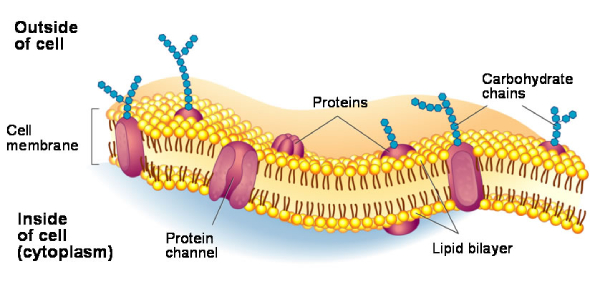
\includegraphics[scale=0.8]{images/1.jpg}

The cell membrane consists of two layers of phospholipids, each containing a head and two tails. The head contains a phosphate group and is hydrophilic and the tails are made up of hydrophobic fatty acids. When these phospholipids combine, they form a bilayer, where the hydrophilic heads face outward, and the hydrophobic tails face inward towards each other. This makes the cell membrane flexible, giving it the ability to change shape. In animal cells, cholesterol is incorporated with the phospholipids. Cholesterol can add flexibility to the membrane, which allows it to adapt to various conditions. The flexibility of the membrane is different in plant cells and is influenced by another lipid, phytosterol. \footnote{Chidrawi et al., 2017}

All membranes have lipid components, which give them flexibility and self-healing properties. Thus, the cells can grow and change shape. During processes like cell division, cell membranes can break and reassemble themselves. The cell membrane and all other membranes inside the cell, including those surrounding organelles, are based on this structure. Then this structure is scattered with proteins. \footnote{Alberts et al., 2002}

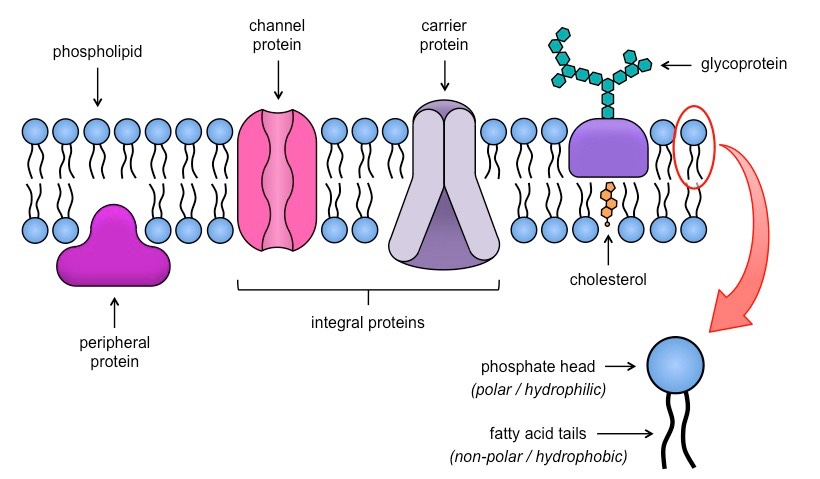
\includegraphics[scale=0.58]{images/2.jpeg}

\subsubsection{Membrane Proteins:}
The plasma membrane contains more than just phospholipids, proteins and lipids are also included within the lipid bilayer, These proteins contribute to the cell membrane's structure and also perform various functions. Many proteins can be used to aid the transport of substances across the cell membrane. \footnote{Chidrawi et al., 2017}

\textbf{Integral Membrane Proteins:}
Integral membrane proteins are embedded within the lipid bilayer. These proteins can serve as a channel for other molecules or receptors for signalling other molecules, or they can serve as enzymes involved in metabolic pathways.

\textbf{Peripheral Proteins:}
Peripheral proteins cling to the membrane's surface rather than being enmeshed in the lipid bilayer. They frequently influence how cells move, shape, and communicate.

\textbf{Cholesterol:} 
Cholesterol molecules are interspersed within the phospholipid bilayer. They help to stabilise the membrane structure by reducing its fluidity at high temperatures and preventing it from becoming too rigid at low temperatures.

\subsubsection{Roles Proteins Provide}
\textbf{Transport pathways and pumps:}
Membrane proteins facilitate the movement of ions, molecules, and nutrients across the cell membrane. Some proteins act as channels, allowing specific substances to pass, while others act as pumps, moving molecules dynamically against increasing concentrations. \footnote{Biology LibreTexts, 2016}

\subsubsection{Cellular signalling and receptors:}
Cellular proteins act as catalysts for signalling molecules such as hormones, neurotransmitters, and growth factors. When these molecules bind to specific cellular responses, such as gene expression, enzyme activation, or changes in cell behaviour. \footnote{Jelokhani-Niaraki, 2022}

\textbf{Enzymatic activity:}
Certain membrane proteins act as enzymes, catalysing biochemical reactions on the cell surface. For example, membrane-bound enzymes are involved in processes such as digestion, energy production, and cellular signalling. \footnote{Jelokhani-Niaraki, 2022}

\textbf{Cell fusion and recognition:}
Intracellular proteins mediate interactions between neighbouring cells and with the extracellular matrix. These interactions are important for tissue integrity, immune response, and cell growth. In addition, membrane proteins help distinguish self from self, allowing immune cells to recognize foreign invaders. \footnote{Zoppi, 2020}

\textbf{Structural Support and maintenance:}
Protein complexes contribute to the stability and shape of the cell membrane. The lipid bilayer is incorporated into the cell structure and provides mechanical strength. The proteins of the outer membrane also play a role in maintaining the inner roundness and organisation of the membrane. \footnote{Biology LibreTexts, 2016}

\textbf{Cell-to-cell interactions and interactions:}
Intracellular proteins participate in cell-to-cell junctions such as complex junctions, desmosomes, and junctions. These interactions allow cells to adhere to each other, share signals, and coordinate activities. For example, gap junction proteins provide direct communication between neighbouring cells by forming channels for ion exchange. (\footnote{Zoppi, 2020}

\subsection{Diffusion}
The simplest way for materials to move across the cell membrane is passive diffusion. During the process of passive diffusion, a molecule goes through the phospholipid bilayer, diffuses across the membrane, and then dissolves into the cytoplasm of the cell, from an area of higher concentration (extracellular fluid) into an area of lower concentration (into the cell). Membrane proteins are not used in this process as molecules are small enough to cross without assistance. Passive diffusion is counted as a selective process because any molecule dissolved in the extracellular fluid can simply enter the cell through the equilibrium of diffusion. The most common substances to enter through passive diffusion are oxygen, water, carbon dioxide, and other small non-charged particles. \footnote{Cooper, 2000}

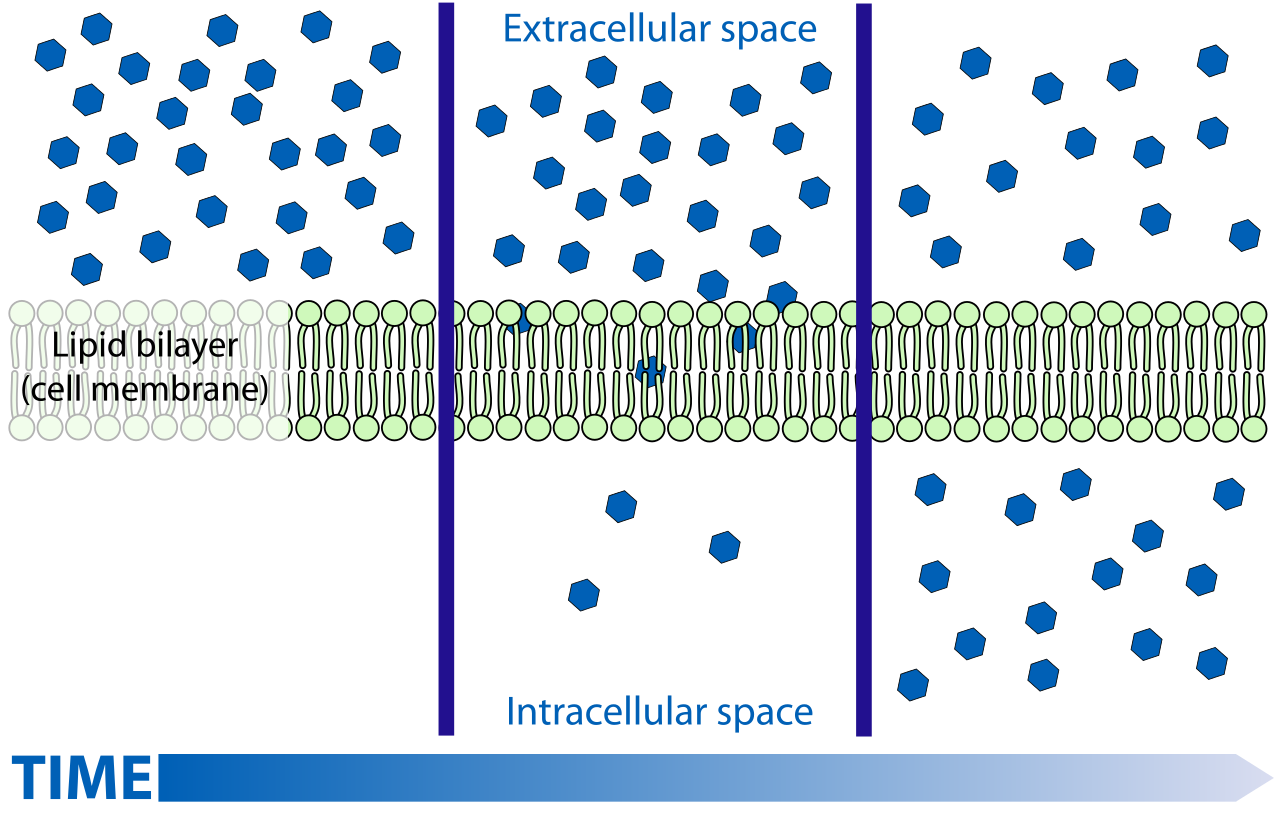
\includegraphics[scale=0.36]{images/3.png}

\subsubsection{Facilitated Diffusion}
Facilitated diffusion, is mainly the same process of diffusion, with it also not requiring any energy source. But facilitated diffusion has a trait that molecules do not simply dissolve in the phospholipid bilayer; instead they are aided by the help of protein channels that allow molecules to pass through the membrane with no interaction from the hydrophobic heads. Two types of proteins allow this function to occur. Carrier proteins and Channel Proteins. \footnote{Cooper, 2000}

\subsubsection{Carrier Proteins}
Carrier proteins are essential for maintaining concentration gradients and regulating the internal environment of cells and are responsible for transporting certain molecules from one side of the membrane to the other. Carrier proteins have a binding site where a specific substance will be recognised eg; ions, sugars, and amino acids, and once bound the carrier protein will receive and undergo a confirmation change that will allow the substance to pass through the membrane. If the cell is moving along the concentration gradient this process will not require any external energy, but if it is moving against the concentration gradient ATP will be used to transport molecules. An example of this is the sodium-potassium pump that maintains sodium and potassium balance in nerve cells. \footnote{BD Editors, 2016} \footnote{Biology Online, 2019}

\subsubsection{Channel Proteins}
Channel Proteins are made up of amino acids which are embedded inside the cell membrane and they serve as a hydrophilic passageway. Channel proteins being integral membrane proteins means that they span across the entire lipid bilayer. Each channel has a specific size and shape which makes it selectively permeable only allowing certain molecules to pass through, and unlike carrier proteins, they remain static in place and generally don't move. Channel proteins serve to provide aid in nerve transmission, muscle contraction, and carrier transport, whilst also helping to regulate cell processes and maintain ion gradients within the cell. \footnote{BD Editors, 2018} \footnote{Editors, 2022}

\subsection{Endocytosis and Exocytosis}
Some molecules are too large to pass through the lipid bilayer or to move through a transport protein, in this stage there are two active transport processes used to transport these macro molecules.

\subsubsection{Endocytosis}
Endocytosis is a process when part the the plasma membrane captures a macro molecule and engulfs it with the cell membrane, where it is surrounded by extracellular space within the cell. The macro molecule then becomes enclosed in a vesicle, which pinches off the membrane and is allowed within the cell. The two main kinds of endocytosis are phagocytosis and pinocytosis. Phagocytosis occurs when the cell engulfs solid material e.g.; bacteria or debris, whereas pinocytosis also called “cellular drinking,” involves the inward folding of the plasma membrane to allow liquids to enter the cell. \footnote{Conner and Schmid, 2003} \footnote{Microbiology Note, 2021}

\subsubsection{Exocytosis}
Exocytosis is the process by which vesicles fuse with the plasma membrane and are able to release their contents from the outside of the cell. Exocytosis most commonly occurs when a cell has produced substances for export, such as newly made proteins and lipids, or waste and toxin products. \footnote{LibreTexts Biology, 2016}

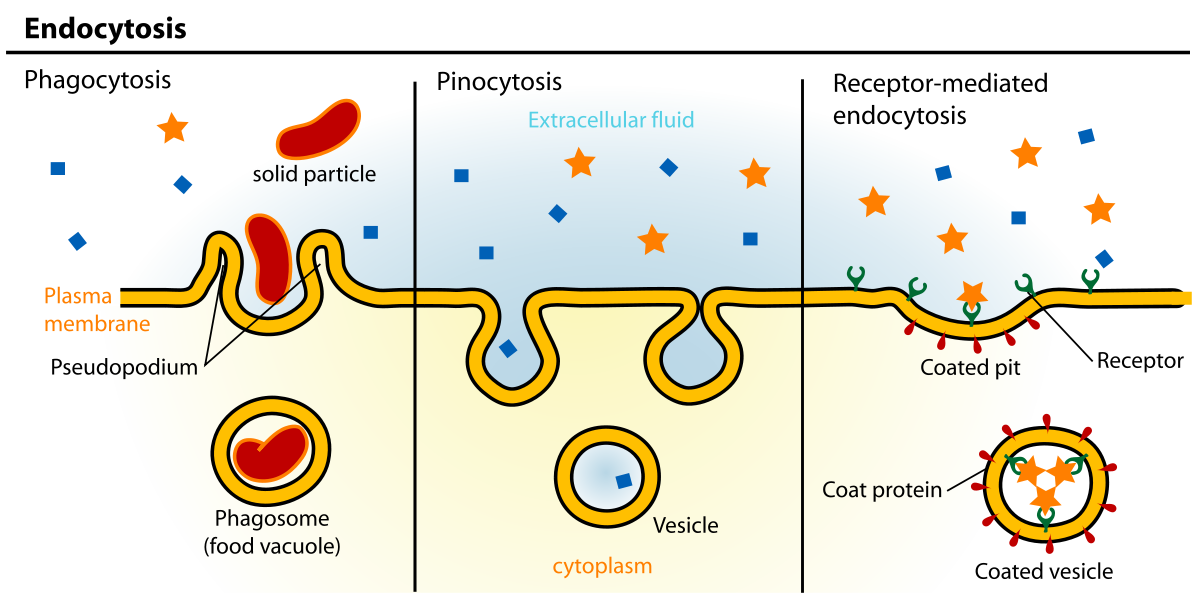
\includegraphics[scale=0.4]{images/4.png}

\subsection{Effect of Cholesterol}
Cholesterol is a lipoprotein, meaning its structure is part lipid and part protein, It serves the purpose of modulating cell membrane fluidity, elasticity, permeability, intracellular transport, signal transduction, and cell trafficking. Made up of the fat called lipoproteins, it displays as a white and waxy substance, essential for cells and carried throughout the bloodstream. 

\subsubsection{Regulation of Fluidity:}
When cholesterol is incorporated into the cell membrane, it reacts with its neighbouring lipids, leading to a tighter packing of lipids within the bilayer, This can lead to stiffness in the membrane. While cholesterol stiffens the membrane, it can prevent any excess rigidity by increasing lipid mobility, which ensures that there is an optimal balance in membrane fluidity. Cholesterol at low temperatures can prevent phospholipids from being tightly packed; this can cause a reduction in membrane rigidity, while at high temperatures, it can restrain excess fluidity, thus causing the membrane to become more stable. This balance ensures optimal and proper membrane function.  \footnote{Zhang, 2019}

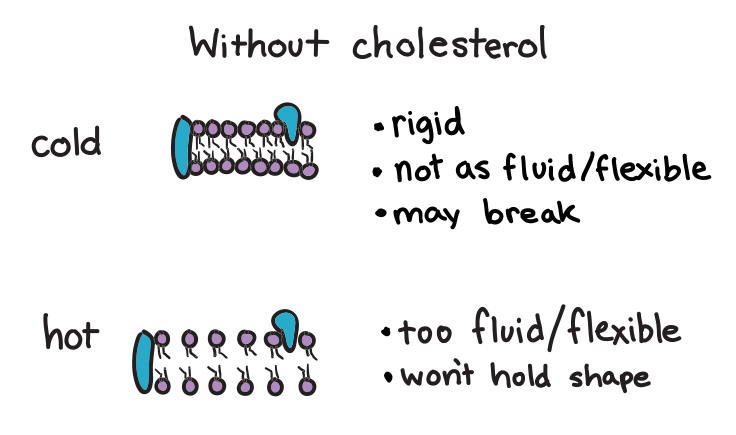
\includegraphics[scale=0.6]{images/6.png}

\subsubsection{Decreased Permeability to Small Water-Soluble Molecules:
}
Cholesterol reduces the permeability of the cell membrane and limits small water-soluble molecules, such as polar molecules and ions. Cholesterol makes the membrane less permeable by filling in the spaces between phospholipid molecules; this is important for maintaining proper osmotic balance of the cell and preventing the leakage of ions needed by the cell

\subsubsection{Enhanced Barrier Function:}
Cholesterol can enhance the lipid bilayer function of the cell membrane against hydrophilic substances. The presence of cholesterol reduces the number of polar molecules crossing through the membrane, which provides an additional layer of protection against non-wanted substances entering the cell. 

\subsubsection{Impact on Membrane Protein Function:}
Cholesterol can have a substantial effect on the functioning of membrane proteins. It can affect the conformation and activity of integral membrane proteins, such as receptors and transporters. The interaction and activity of these molecules can modulate and consequently affect the permeability of the lipid bilayer to certain molecules.

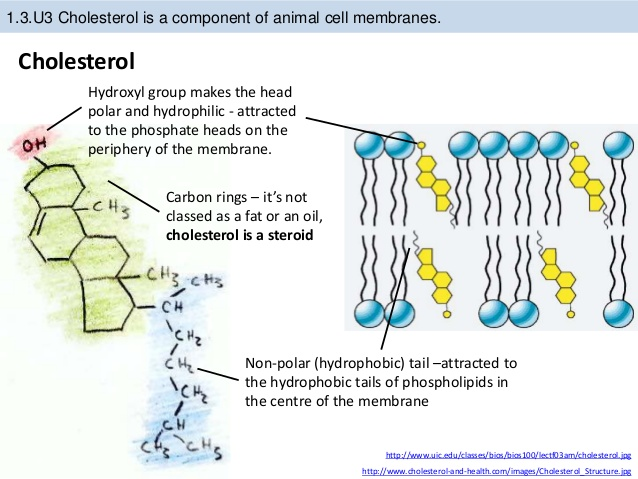
\includegraphics[scale=0.7]{images/5.jpg}

\newpage

\section{Cholesterol and Beetroot Membrane Permeability Experiment}
\section{AIM}
To investigate the effect of temperature and cholesterol (salt) on the permeability of beetroot cell membranes. By examining the amount of betalain pigment leakage from the beetroot into its surrounding solutions. \footnote{Abola, 2020}

\section{Hypothesis}
\begin{theorem}
Cholesterol plays a crucial role in regulating cell membrane permeability. It is hypothesised that an ideal temperature and optimal cholesterol concentration will enhance membrane stability and reduce permeability. However, deviations from this ideal range, either excess or undersupply of cholesterol, may disrupt the balance of permeability, severely impacting the movement of molecules in the membrane. If the hypothesis is proven false, it would suggest that cholesterol levels in the cell membrane have minimal impact on overall permeability, regardless of temperature variations. \footnote{Eduqas UK, 2021} \footnote{Isa, 2017}
\end{theorem}

\section{Risk Assessment}
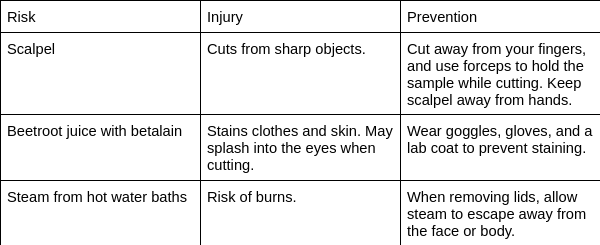
\includegraphics[scale=0.8]{images/risk_table.png}

\section{Materials}
\begin{itemize}
    \item 2 x Red beetroot
    \item 1 x Knife
    \item 1 x Cutting Board
    \item 1 x Thermometer
    \item 4 x 500ml Beaker
    \item 4 x 20 x 20 cm Dish
    \item 1 x Kettle
    \item 1 x Stirring Rod
    \item 1 x Salt 100g
    \item 1 x 1L Water
    \item 1 x Gloves
    \item 1 x Lab Coat
    \item 1 x Goggles
\end{itemize}

\section{Method}
\begin{enumerate}
    \item Wear all PPE, such as gloves, lab coat, and goggles.
    \item Cut the beetroot into 4 uniform 2cm x 2cm x 1cm slices using a knife.
    \item Boil approximately 1 liter of water.
    \item Use a thermometer to measure the temperature of the boiled water, and wait until the temperature reaches 40 °C.
    \item Lay out 2 20cm x 20cm dishes and label each appropriately, ‘Salt Solution’ and ‘Water Solution’, additionally, mark which solution will be hot or cold water.
    \item Add 250 ml of hot water to the ‘Salt Solution’ container, and add 50 grams of salt. Mix thoroughly until dissolved.
    \item Add 250 ml of room temperature water to the ‘Water Solution’ container.
    \item Add 1 slice of beetroot to each container and wait 5-10 minutes.
    \item Document the amount of betalain (pigment) released from each solution.
    \item Go back to step 5 and repeat, but this time use cold water for your ‘Salt Solution’ and hot water for the ‘Water Solution’
    \item Repeat the experiment as many times as you feel is necessary.
\end{enumerate}

\section{Results}
\subsection{Betalain Leakage}
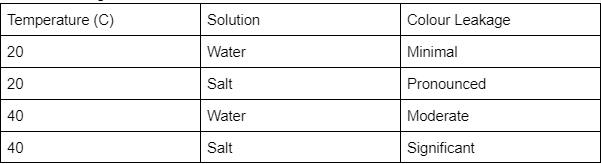
\includegraphics[scale=1]{betalain_leakage.png}

\subsection{Colorimeter Readings}
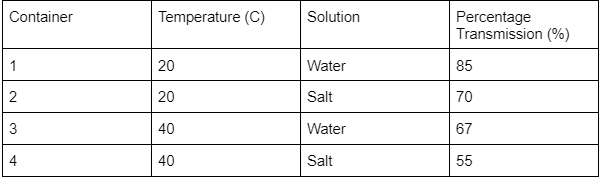
\includegraphics[scale=1]{colourimeter_percentage.png}

\subsection{Colorimeter Reading Graph}
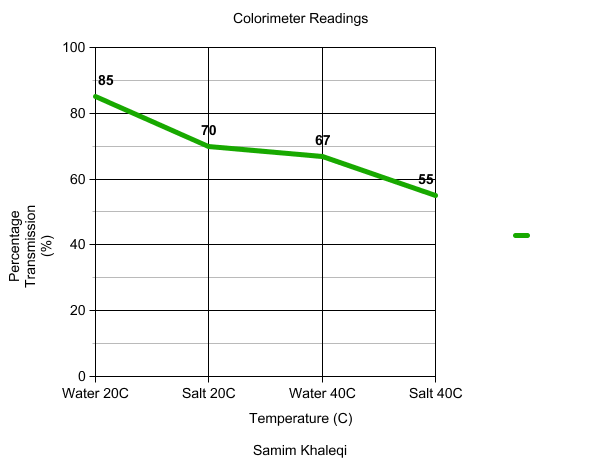
\includegraphics[scale=0.8]{images/colourimeter_graph.png}

\begin{figure}
    \centering
    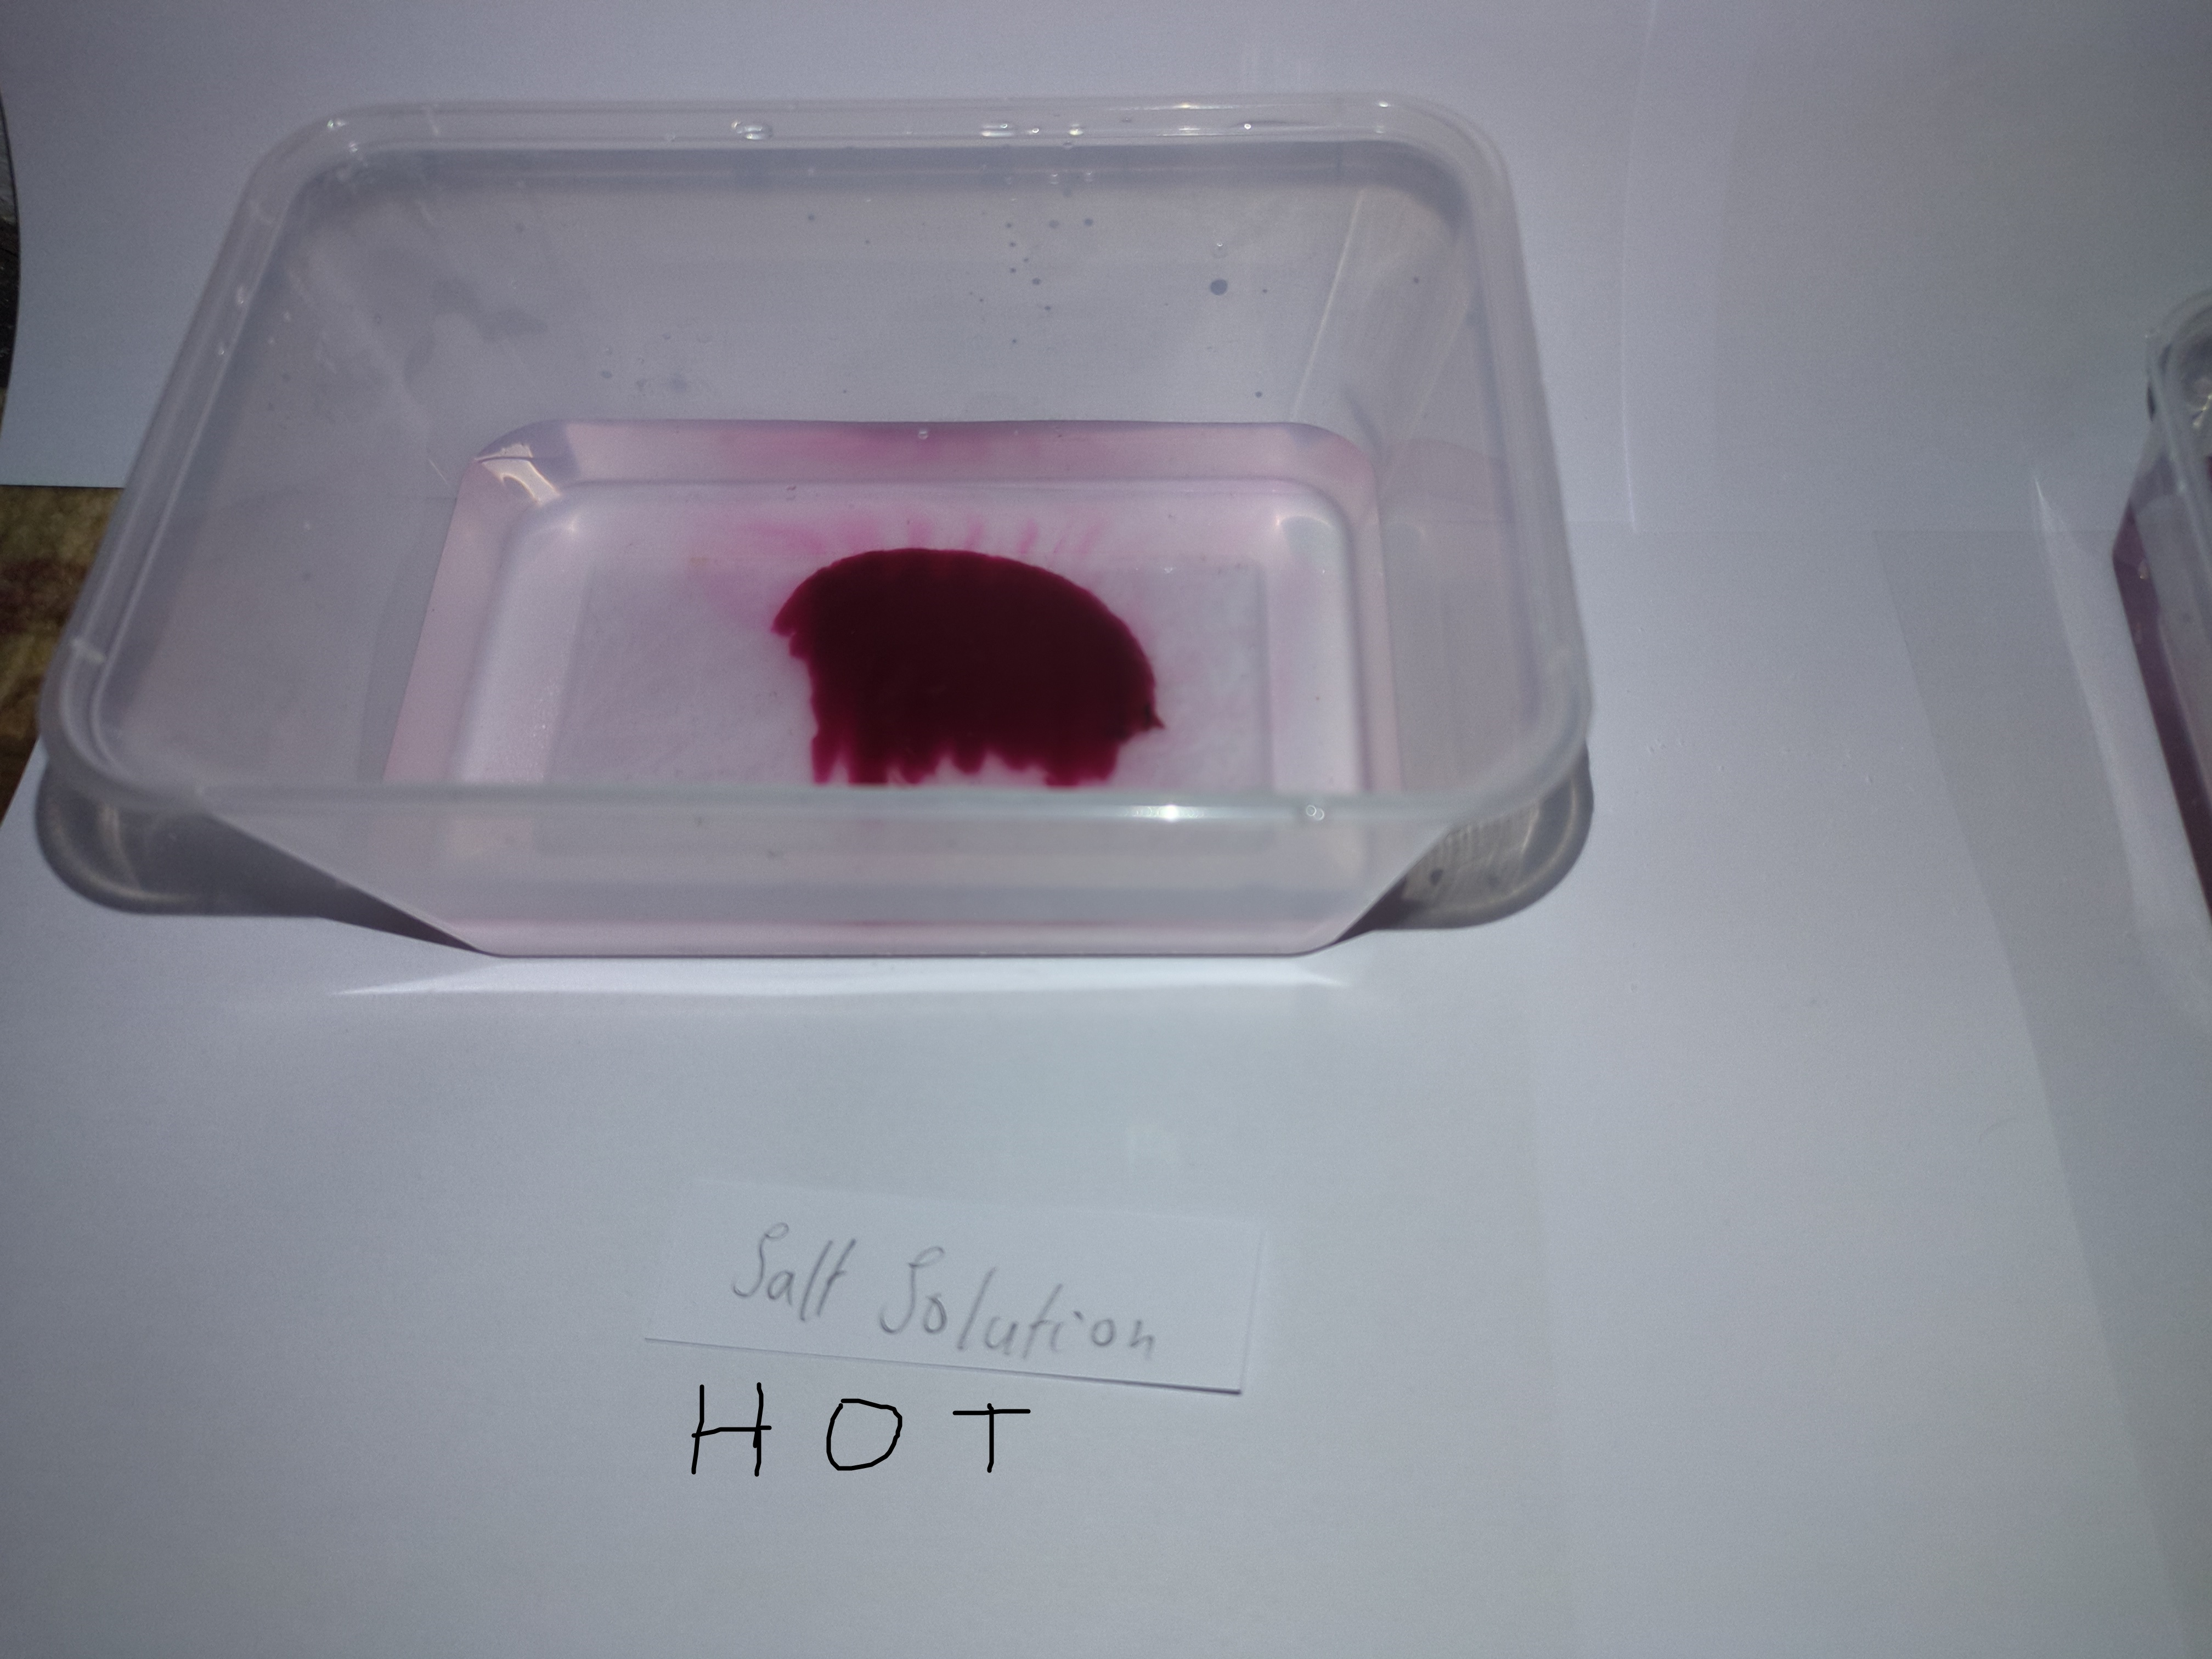
\includegraphics[scale=0.1]{images/P_0.jpg}
    \caption{Beetroot after 10 minutes in a hot salt solution }
    \label{fig:enter-label}
\end{figure}

\begin{figure}
    \centering
    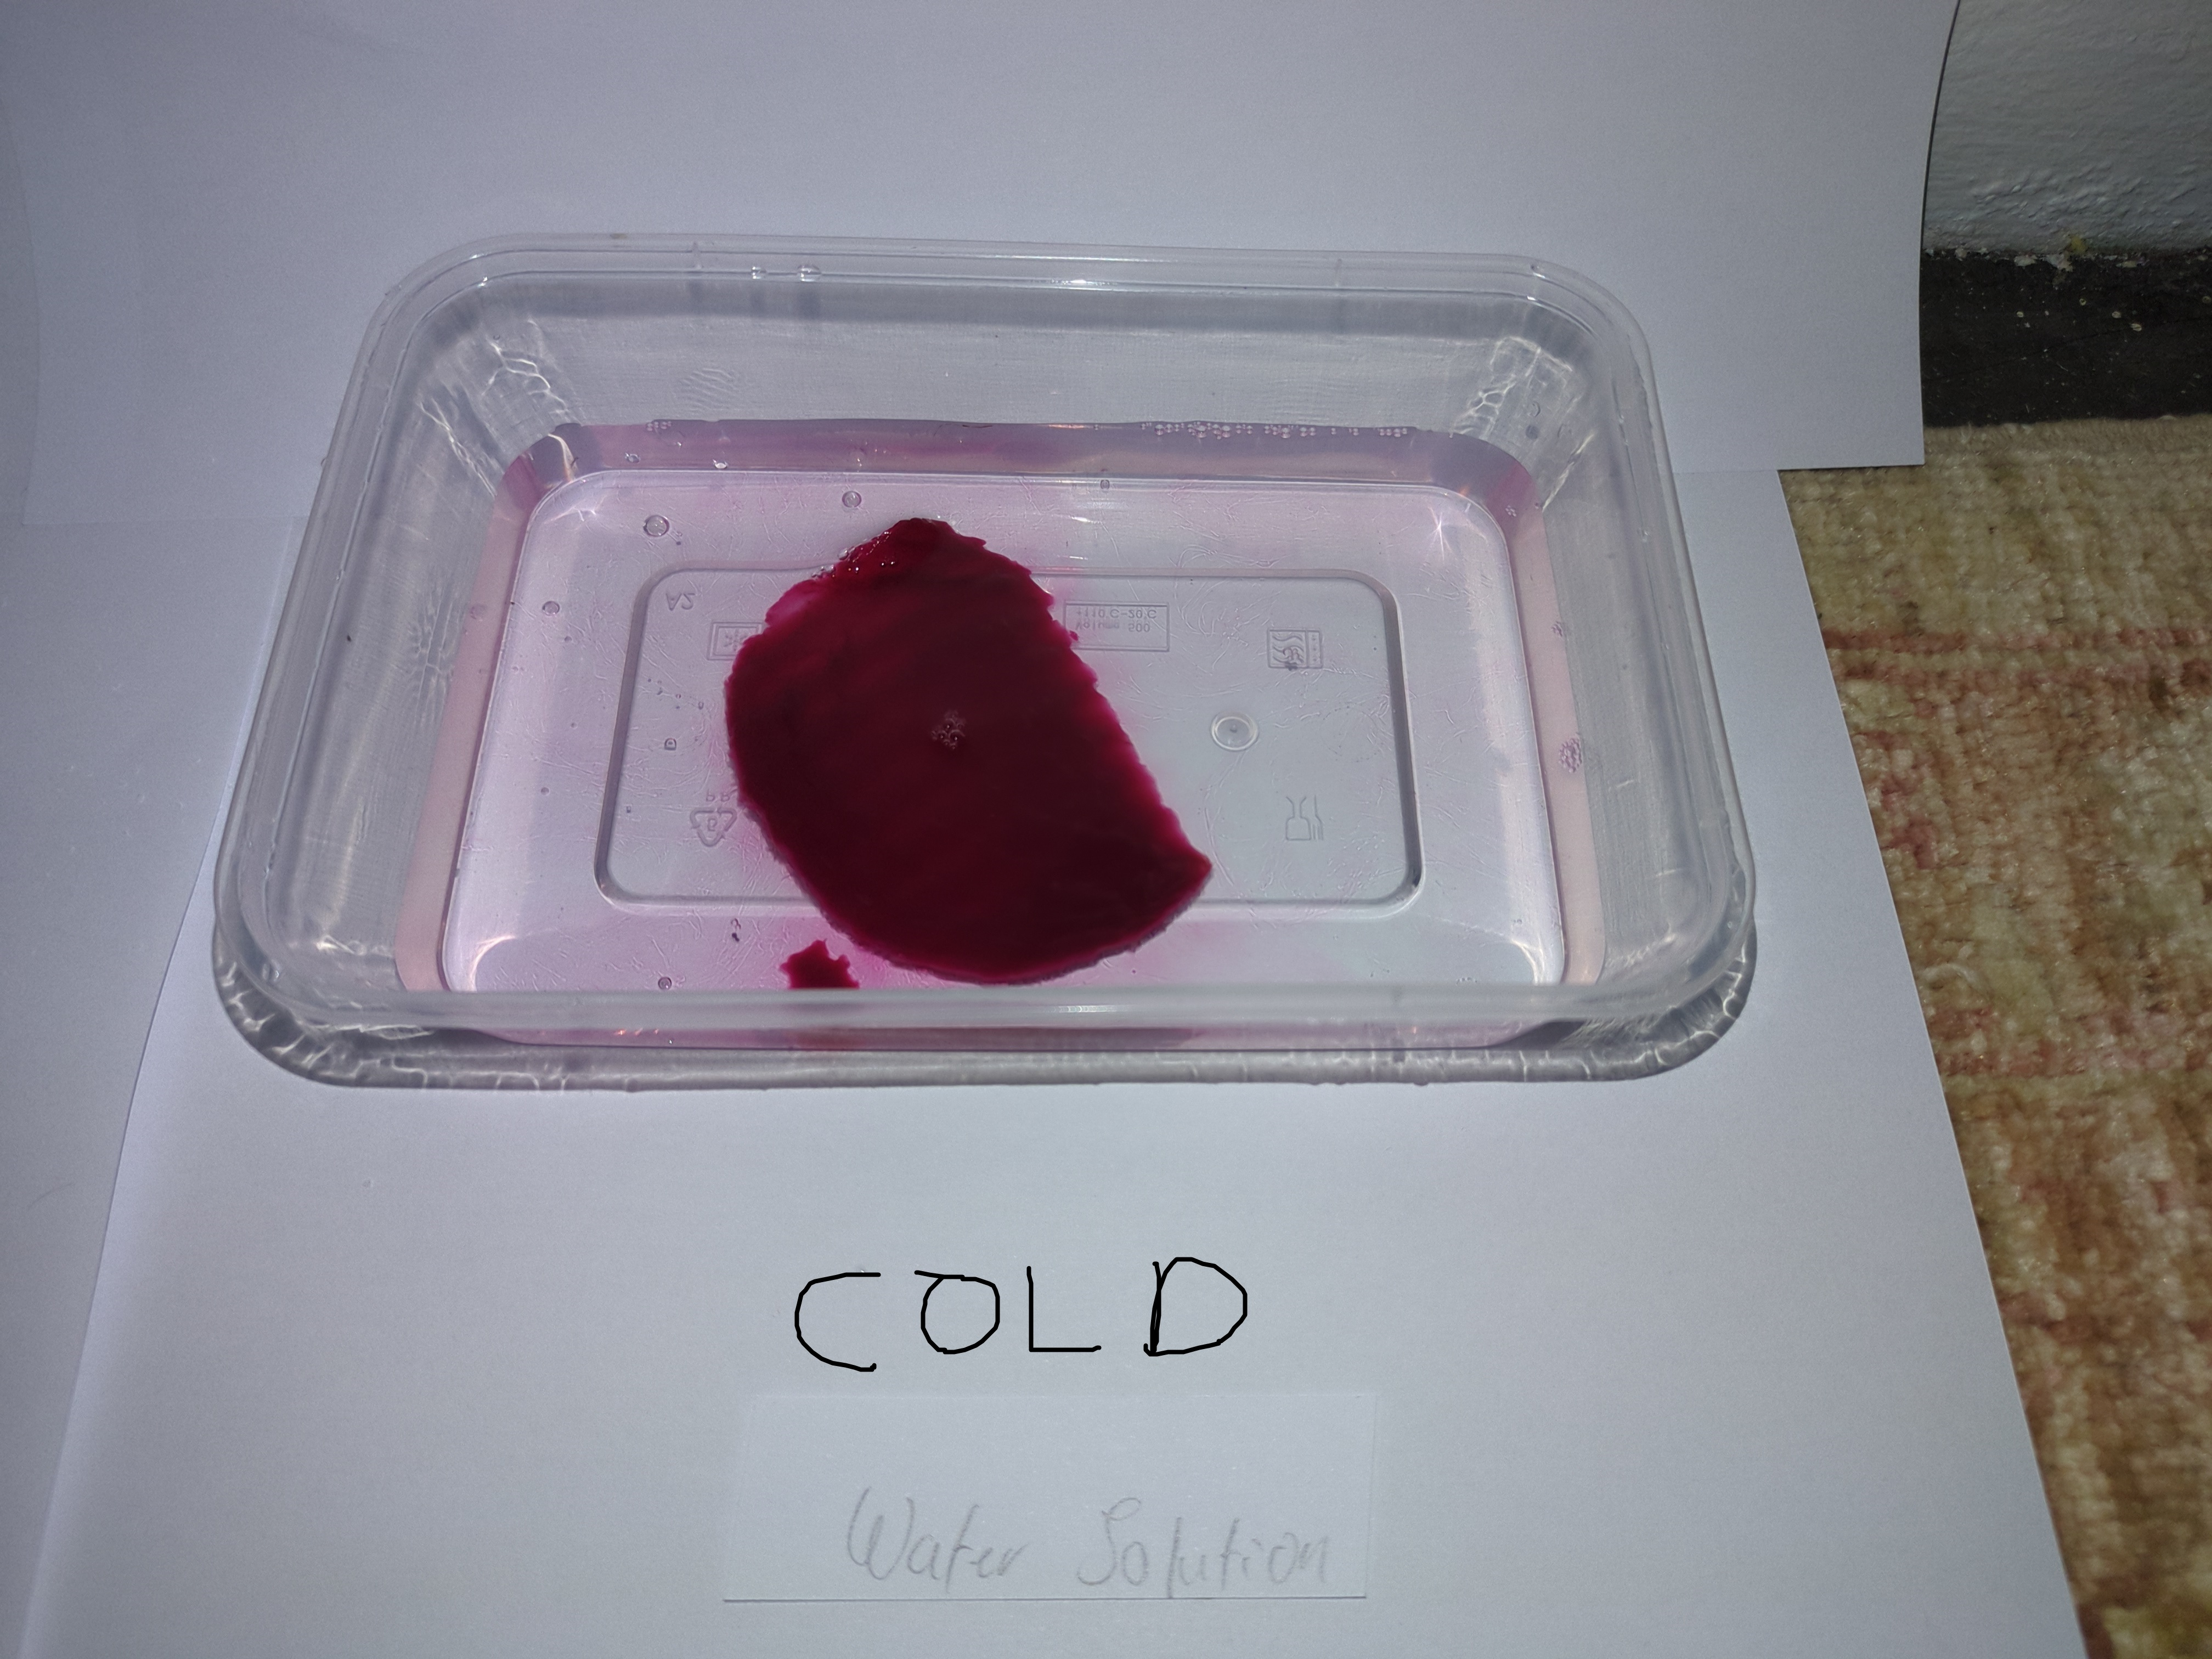
\includegraphics[scale=0.1]{images/P_1.jpg}
    \caption{Beetroot after 10 minutes in a cold water solution, notice the amount of betalain released}
    \label{fig:enter-label}
\end{figure}

\begin{figure}
    \centering
    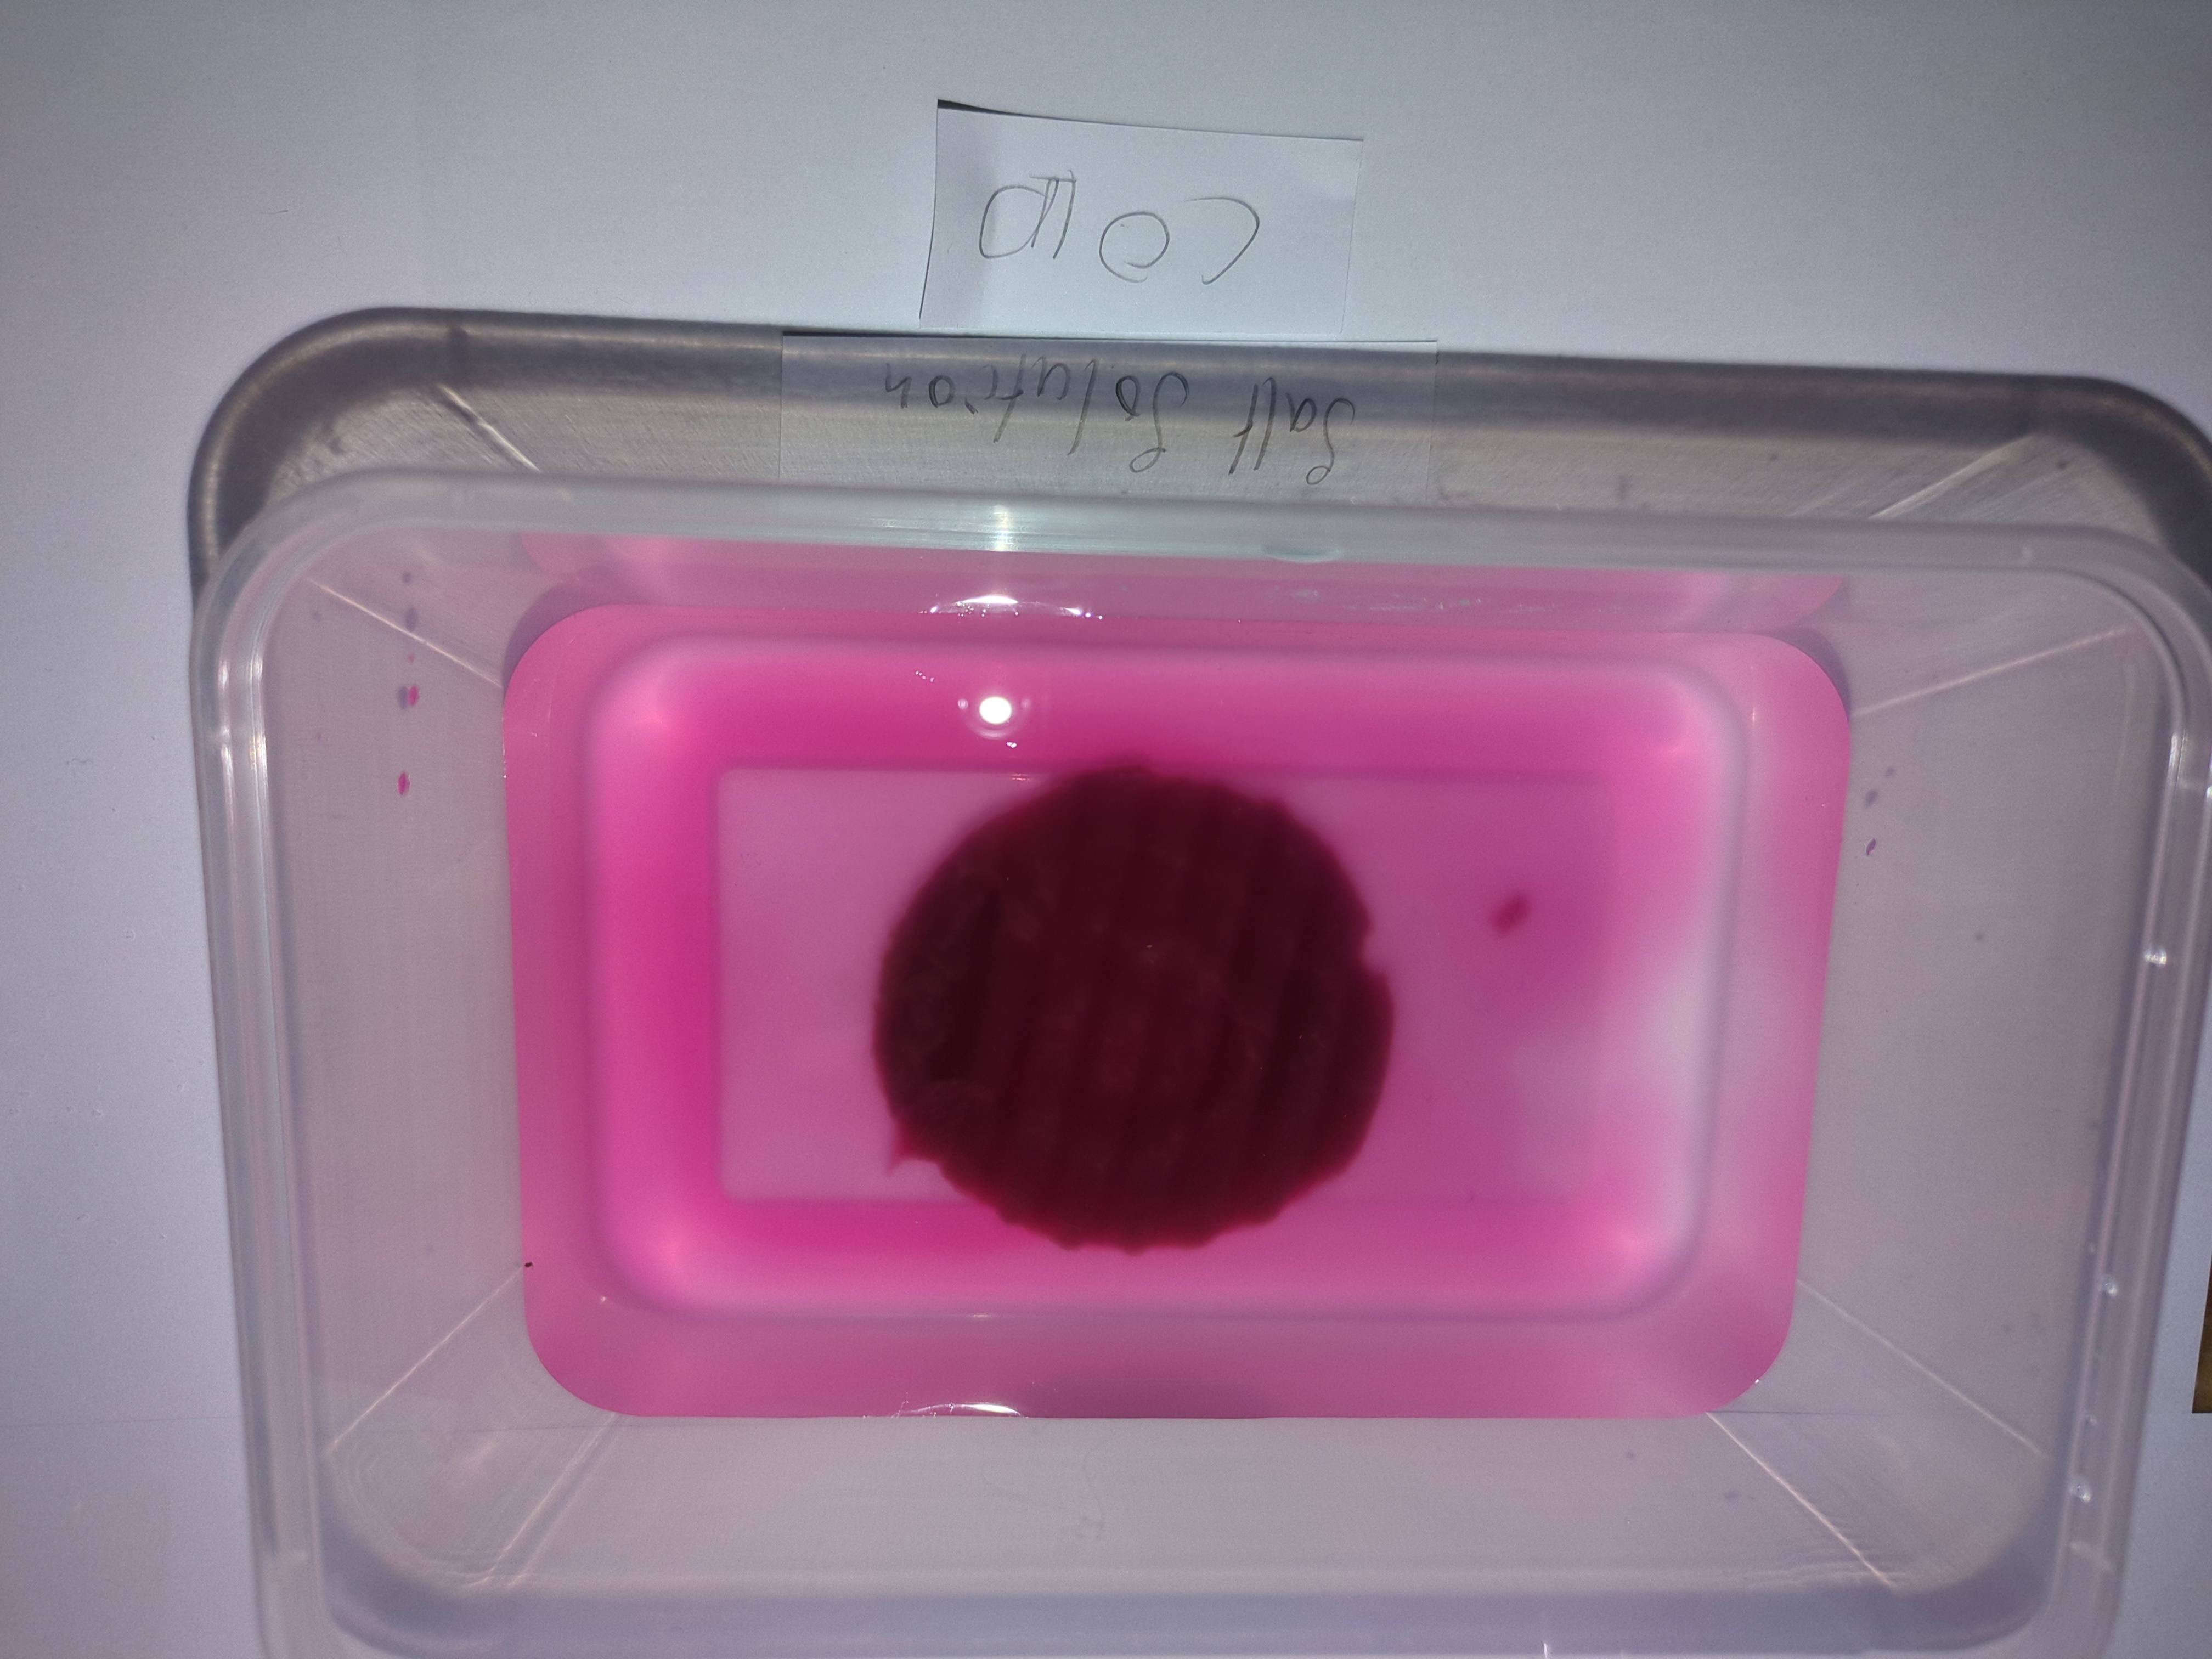
\includegraphics[scale=0.1]{images/P_4.jpg}
    \caption{Beetroot after 10 minutes in a cold salt water solutuion}
    \label{fig:enter-label}
\end{figure}

\begin{figure}
    \centering
    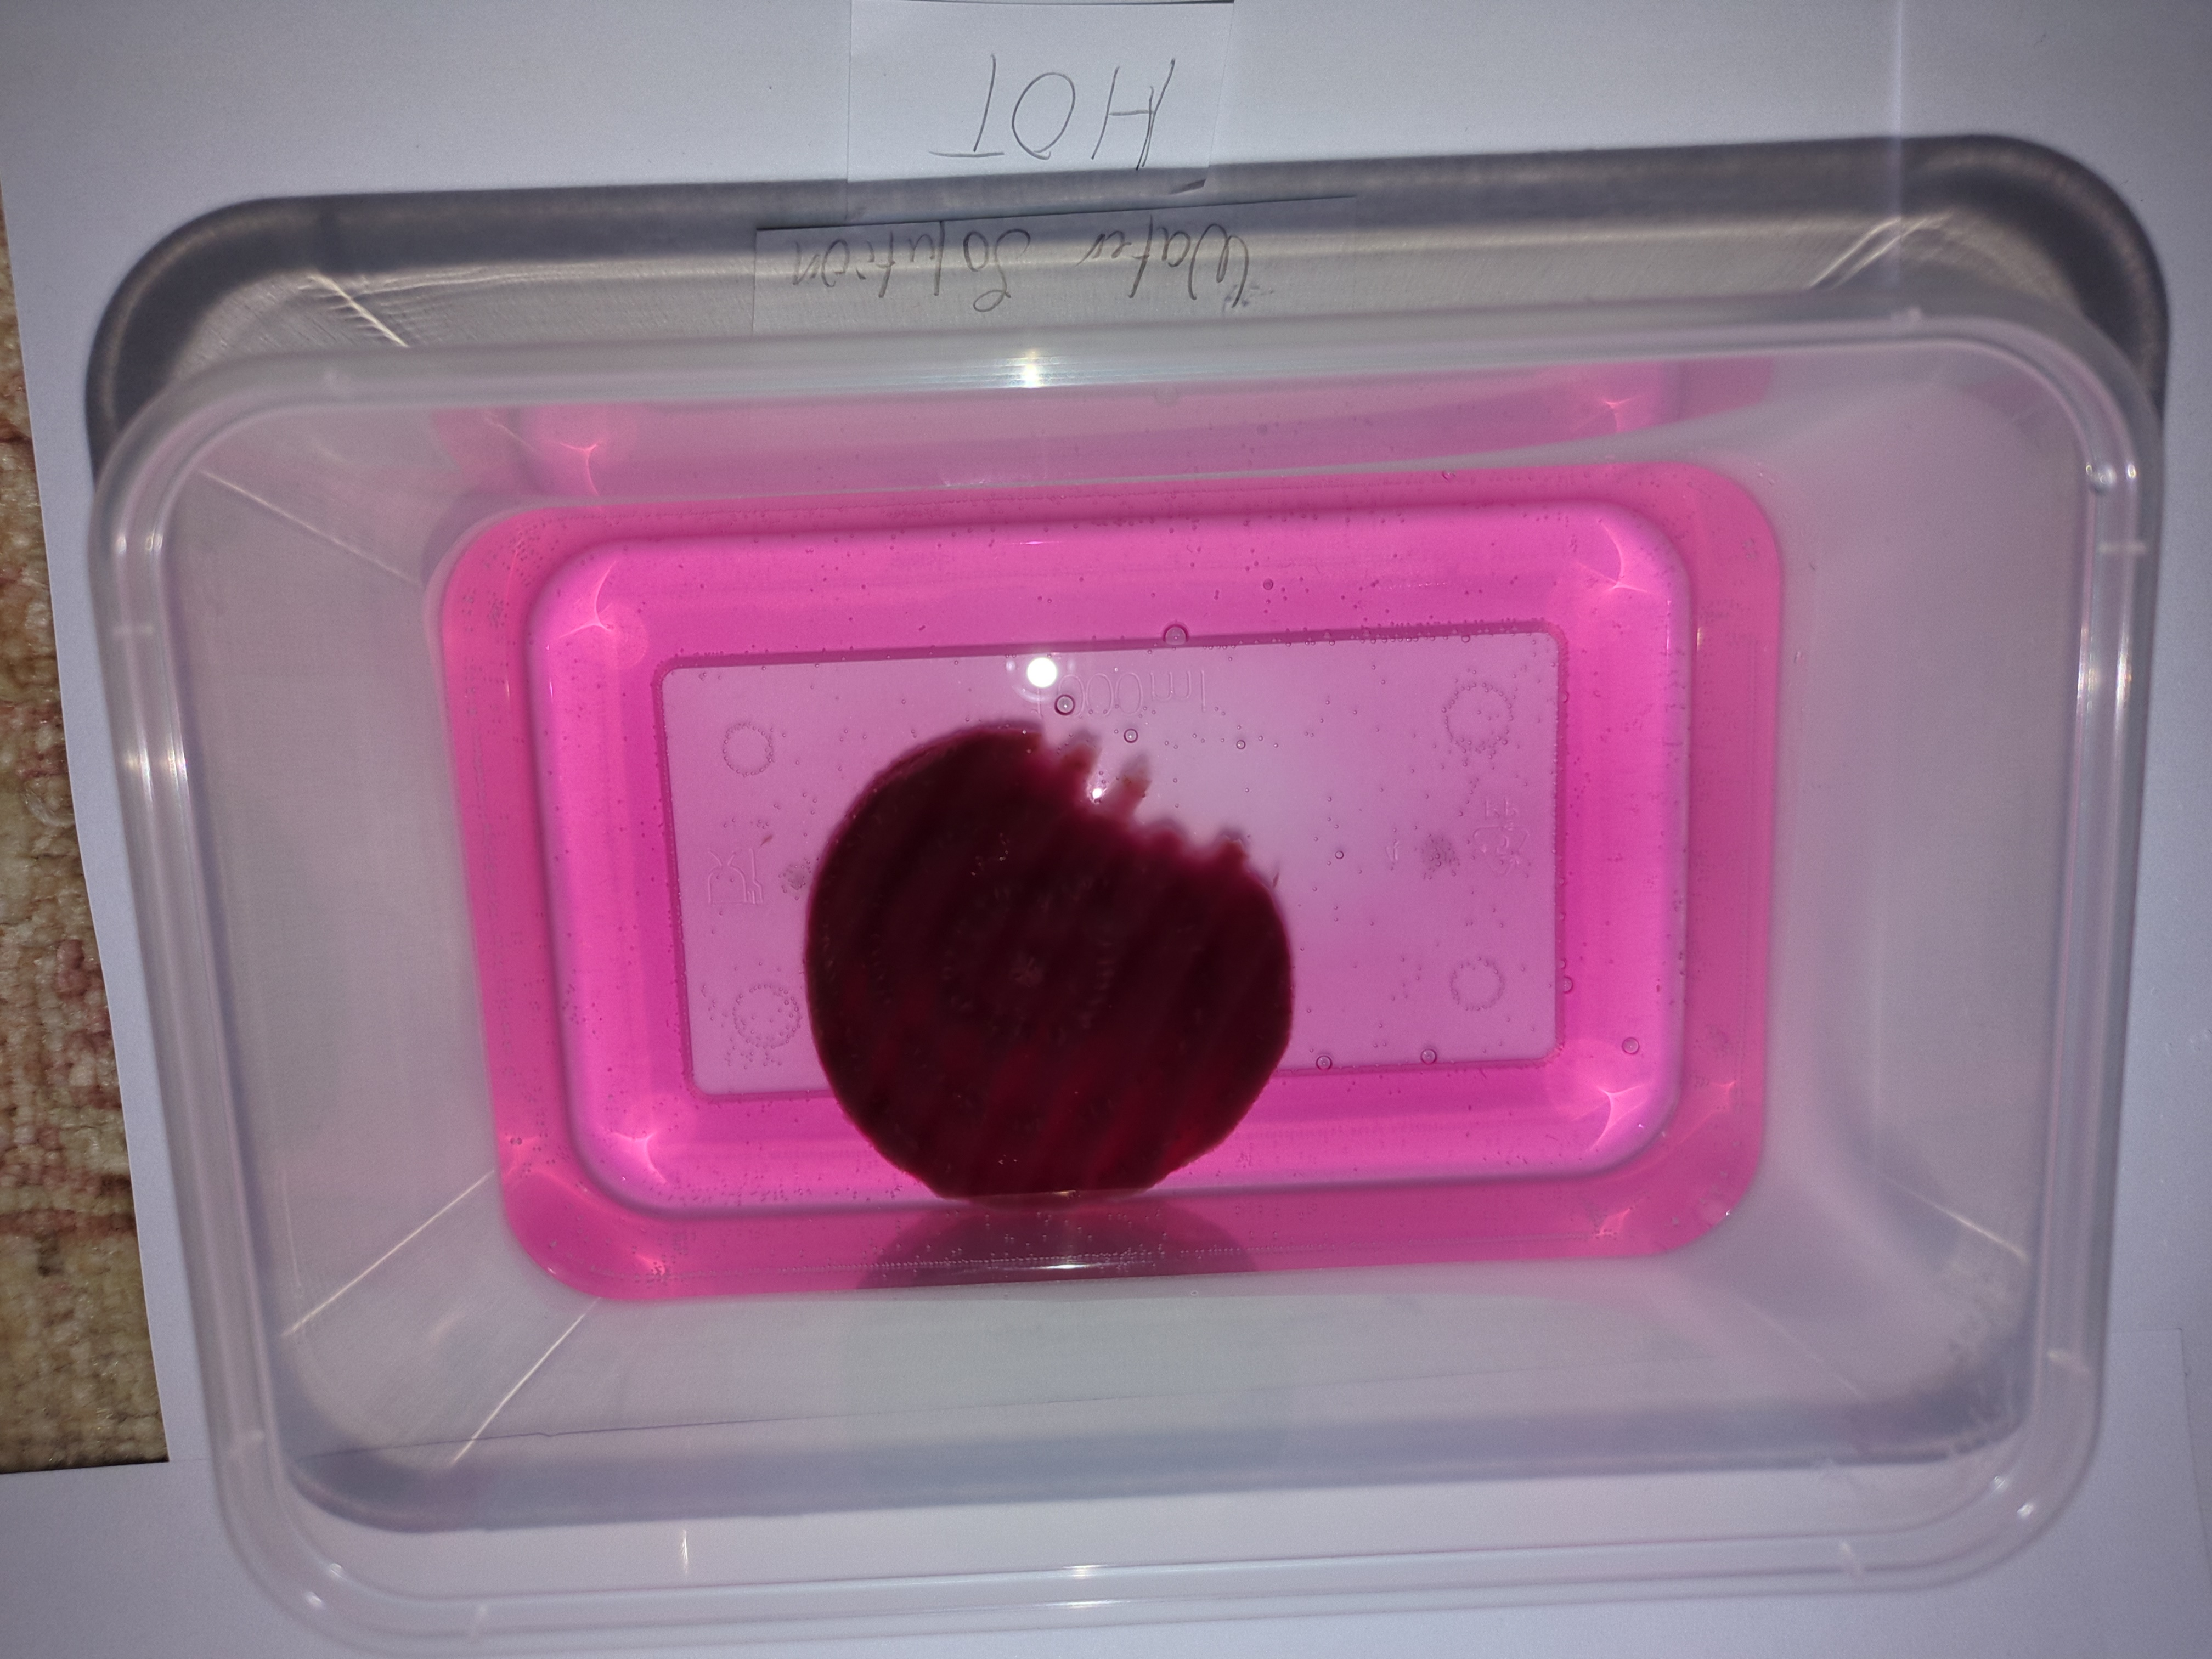
\includegraphics[scale=0.1]{images/P_5.jpg}
    \caption{Beetroot after 10 minutes in a hot water solution, notice the amount of betalain released even though there is no catalyst such as salt}
    \label{fig:enter-label}
\end{figure}

\section{Discussion}
The results provided from the experiment showed us that our hypothesis was correct, stating that our cholesterol (salt) caused an impact on cell membrane permeability, as seen by the result of pigmentation release being more substantial in the salt solutions. Temperature also proved successful, as at higher temperatures, there was more release of betalain when compared to the room temperature solutions. These results show such:

\subsection{Effect of temperature}
At both temperatures, it was observed that there was a decrease in percentage transmission, which indicates that there was an increase in betalain release when beetroot slices were placed in a salt solution when compared to a water solution. This shows that in higher temperatures, the permeability of beetroot cell membranes is enhanced, which allows more betalain to be released.

\subsection{Salt Solution Influence}
The presence of salt at both temperatures showed a further increase in cell membrane permeability, this can be seen in \textbf{FIG 1}. This is due to how salt disrupts the lipid bilayer, therefore making it more porous and allowing betalain molecules to leak out of the cell.

\subsection{Consideration of Cholesterol}
While the effect of cholesterol was not directly investigated in this experiment, it is still applicable to this experiment. The salt solution is used to substitute for the cholesterol solution because it also affects cell membrane permeability. Whereas cholesterol maintains membrane fluidity and stability, salt can have an osmotic effect, This is when cells are exposed to a hypertonic solution, which causes water to move out of a cell, This process causes cell damage as the cell shrinks, leading to membrane damage, though this increase in salt concentration does lead to a more permeable membrane, as seen in how cholesterol affects the cell membrane in hypertonic solutions. \footnote{Biology LibreTexts, 2018}

\subsection{Temperature-dependent permeability}
Temperature-dependent permeability refers to how the permeability of cell membranes is affected by temperature. As temperature increases, the lipid bilayer of a cell becomes more fluid, this fluidity can affect how lipids and proteins are arranged within this bilayer, so at higher temperatures, the lipid bilayer can move more freely, which enables a greater ability for permeability. This is shown in FIG. (x), where in the hot water solution, the pigmentation of water was shown to be greater. This proves that temperature has a direct correlation with the permeability of the cell membrane.

\subsection{Limitations of the Experiment}
While this experiment only focused on beetroot cell membranes and their permeability, this may not apply to all cell types. In future experiments, it would be beneficial to explore the specific role of cholesterol and any other related factors in how it affects cell membrane permeability. Another factor that influenced the direction of this experiment was Bellfield College, as requests for more in-depth and informative experiments were shut down due to red blood cells being “unsafe” for student research. If red blood cells were used and the acquisition of 3B-Hydroxy-5-cholestene and L-a-Phosphatidylcholine were successful, a more coherent and comprehensive study could be conducted, but unfortunately not today.

\section{Conclusion}
In this investigation, we measure beetroot cell membrane permeability by using factors such as temperature and a simulation of cholesterol using salt. The following temperatures (20C and 40C) were used in this experiment, and the pigmentation of betalain was observed using both a hypertonic salt solution and a plain water solution. This experiment found that under higher temperatures and higher salt concentrations, the cell membrane permeability barrier significantly increased, causing hyper pigmentation of the external liquid surrounding the beetroot, answering the hypothesis that an oversupply of cholesterol will cause an imbalance in cell membrane permeability, which will severely affect the movement of molecules within a cell membrane.

\newpage
\section{Acknowledgements}
The authors would like to thank Mrs Saja Bashier for her help in class and for providing the author with relevant information to complete this in-depth study and Lucia Lowe from Creative Biolabs.
The author would also like to acknowledge the peers who helped review, clarify, and provide information on this study.
A final acknowledgment can be made of the author's dreams, where they received divine revelations from Allah (SWT) about this in-depth study and what to include within this study.


% Bibliography
\clearpage
\pagestyle{\auxsettings}
\printbibliography[heading=bibintoc]
\end{document}
